\section{Überschriften}
%Bis hier im Inhaltsverzeichnis
\subsection{Unterüberschrift 1}
\subsubsection{Unterunterüberschrift 2}
%Alles darunter: Passt Struktur?!
\paragraph{Unterunterunterüberschrift 3}
\subparagraph{Unterunterunterunterüberschrift 4}

% \\ Ist ein Zeilenumbruch
\section{Formatierungen}
\textbf{Fetter Text} \\
\textit{Kursiver Text} \\
\texttt{Computer Text} \\
\underline{Unterstrichener Text} \\
\emph{Hervorgehoben} \\

% \verb kann Latex Text wortwörtlich ausgeben und nicht verarbeiten
Der Text \verb|textbf{}| wird fett geschrieben

\begin{verbatim}
    %Abschnitt für \verb
\end{verbatim}

%Beispieltext ist auch rot, Farbe zieht sich so weiter
\color{red}{Roter Text} \\
Beispieltext

%Setzt nur diesen Text auf die Farbe, der Beispieltext bleibt jedoch rot, wegen dem Weiterziehen von oben
\textcolor{blue}{Blauer Text}
Beispieltext

%Unterbinden mit geschweiften Klammern, Farbe nur in diesem Abschnitt
{
    \color{green}{grüner Text}
}

\section{Schriftgrößen}
{\tiny Tiny Text} \\
{\scriptsize Scriptsize Text} \\
{\footnotesize Footnotesize Text} \\
{\small Small Text} \\
{\normalsize Normalsize Text} \\
{\large Large Text} \\
{\Large Large Text} \\
{\LARGE LARGE Text} \\
{\huge Huge Text} \\
{\Huge HUGE Text} \\

\section{Textausrichtungen}
\begin{center}
    Zentrierter Text
\end{center}

\begin{flushleft}
    Linksbündiger Text
\end{flushleft}

\begin{flushright}
    Rechtsbündiger Text
\end{flushright}

\section{Listen}
\begin{itemize}
    \item Aufzählungspunkt 1
    \item Aufzählungspunkt 2
    \begin{itemize}
        \item Unterpunkt 1
        \item Unterpunkt 2
    \end{itemize}
    \item Aufzählungspunkt 3
\end{itemize}

\begin{enumerate}
    \item Nummerierter Punkt 1
    \item Nummerierter Punkt 2
    \begin{enumerate}
        \item Unterpunkt 1
        \item Unterpunkt 2
    \end{enumerate}
    \item Nummerierter Punkt 3
\end{enumerate}

\section{Sonderzeichen}
\&, \%, \$, \#, \_, \{, \}, \textbackslash, \textasciitilde, \textasciicircum

%Anführungszeichen doppelt oben
Dieser Text ist unter Anführungzeichen gesetzt: ``Beispieltext''. \\

%Anführungszeichen deutsch, unten und oben
Dieser Text ist unter Anführungzeichen gesetzt: \glqq Beispieltext \grqq. \\

%Anführungszeichen einfach, unten und oben
Dieser Text ist unter Anführungzeichen gesetzt: \glq Beispieltext \grq.

%c/m definieren, wo vertikale Linie gezogen werden
%hline definiert horizontale Linie
%c Standardmäßige Größe
%m Breitendefinition
\section{Tabellen}
\begin{tabular}{|c|m{5cm}|c|}
    \hline
    Spalte 1 & Spalte 2 & Spalte 3 \\
    \hline
    Eintrag 1 & Eintrag 2 & Eintrag 3 \\
    Eintrag 4 & Eintrag 5 & Eintrag 6 \\
    \hline
\end{tabular}
% IST NICHT IM TABELLENVERZEICHNIS

%h -> here platzieren wenn möglich
%! -> überschreibt X-Parameter
%H -> zwingend here platzieren
%T -> zwingend top platzieren
%B -> zwingend bottom platzieren
\begin{table}
    \centering
    \begin{tabular}{|c|m{5cm}|c|}
        \hline
        Spalte 1 & Spalte 2 & Spalte 3 \\
        \hline
        Eintrag 1 & Eintrag 2 & Eintrag 3 \\
        Eintrag 4 & Eintrag 5 & Eintrag 6 \\
        \hline
    \end{tabular}
    \caption{Beispieltabelle}
    \label{tab:beispieltabelle}
\end{table}
Wie in der Tabelle \ref{tab:beispieltabelle} zu sehen ist, handelt es sich hier um eine Beispieltabelle.
%IST IM TABELLENVERZEICHNIS -> beginn{table}
% Nummerierung: [Nr1].[Nr2] -> Nr1 Kapitelnummer, Nr2 Tabellennummer im Kapitel

%RELATIVE GRÖßE
%width=0.5\textwidth -> Hälfte der Bildschirmbreite
\section{Abbildung}
\begin{figure}[H]
    \centering
    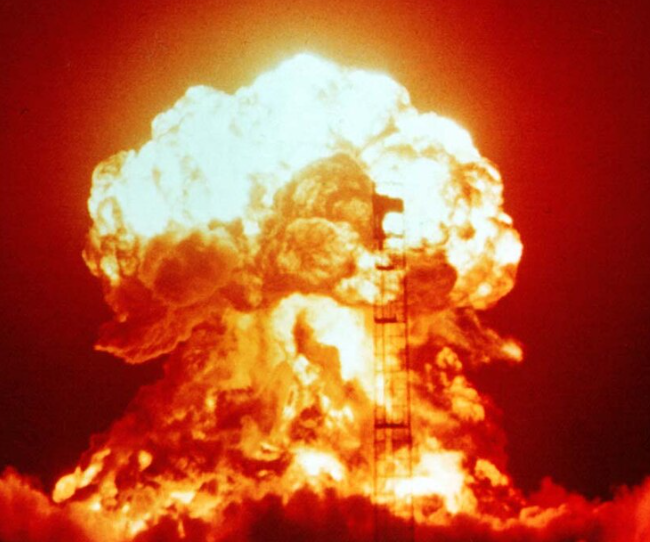
\includegraphics[width=0.5\textwidth]{content/img/3_prototype/Bild.png}
    \caption{Beispielbild}
    \label{fig:beispielbild}
\end{figure}
Wie in der Abbildung \ref{fig:beispielbild} zu sehen ist, handelt es sich hier um ein Beispielbild.

%ABSOLUTE GRÖßE
%width=5cm -> 5 Zentimeter Breite
%angle=90 -> 90 Grad Drehung
\section{Abbildung}
\begin{figure}[H]
    \centering
    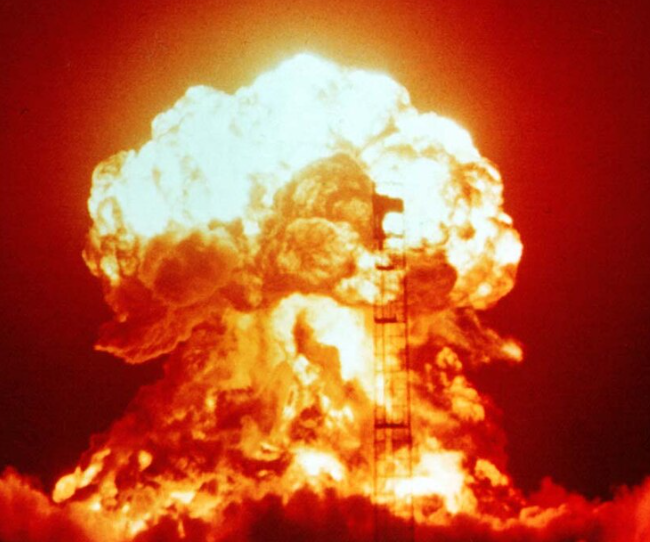
\includegraphics[width=5cm, angle=90]{content/img/3_prototype/Bild.png}
    \caption{Beispielbild}
    \label{fig:beispielbild2}
\end{figure}
Wie in der Abbildung \ref{fig:beispielbild2} zu sehen ist, handelt es sich hier um ein Beispielbild.

%Noch nicht schön formatiert -> /section/packages.tex -> können für Code Formatierungen angelegt werden (Farben, usw.)
\section{Code}
\begin{lstlisting}[language=Python, caption={Beispiel Python Code}, label={lst:beispielpythoncode}]
def beispiel_funktion(parameter1, parameter2):
    # Dies ist ein Kommentar
    ergebnis = parameter1 + parameter2
    return ergebnis
print(beispiel_funktion(5, 10))
\end{lstlisting}
%/content/src kann man Code auslagern -> schöner

%PDF includen -> /6_appendix/meetingMinutes.tex

\section{Formeln}
Hier eine Beispiel-Formel für den Satz des Pythagoras:
\begin{equation}
    a^2 + b^2 = c^2
\end{equation}

%Akronym & Glossar Definition -> /setup/glossaracronyms.tex
%Akronym & Glossar Verwendung -> /3_protoype/description.tex